\chapter{ĐO PROFILE}

\section{Mục đích}
\begin{itemize}
	\item Giúp sinh viên nắm vững các kỹ năng đo và kiểm tra các sai lệch hình học.
	\item Sinh viên được thực hành trên máy đo profile của MITUTOYO hiện đại và chính xác.
\end{itemize}

\section{Báo cáo}
Nhận xét:
\begin{itemize}
	\item Các kích thước thực là số lẻ bởi vì sai số của phép đo. Trong trường hợp này là máy đo profile và người thí nghiệm. Qua các kích thước ta có thể xây dựng được bản vẽ.
	\item Một số giả định được đưa ra để dễ đo đạc (ví dụ như độ vuông góc, đồng tâm,...)
\end{itemize}
\begin{figure}[ht]
	\centering
	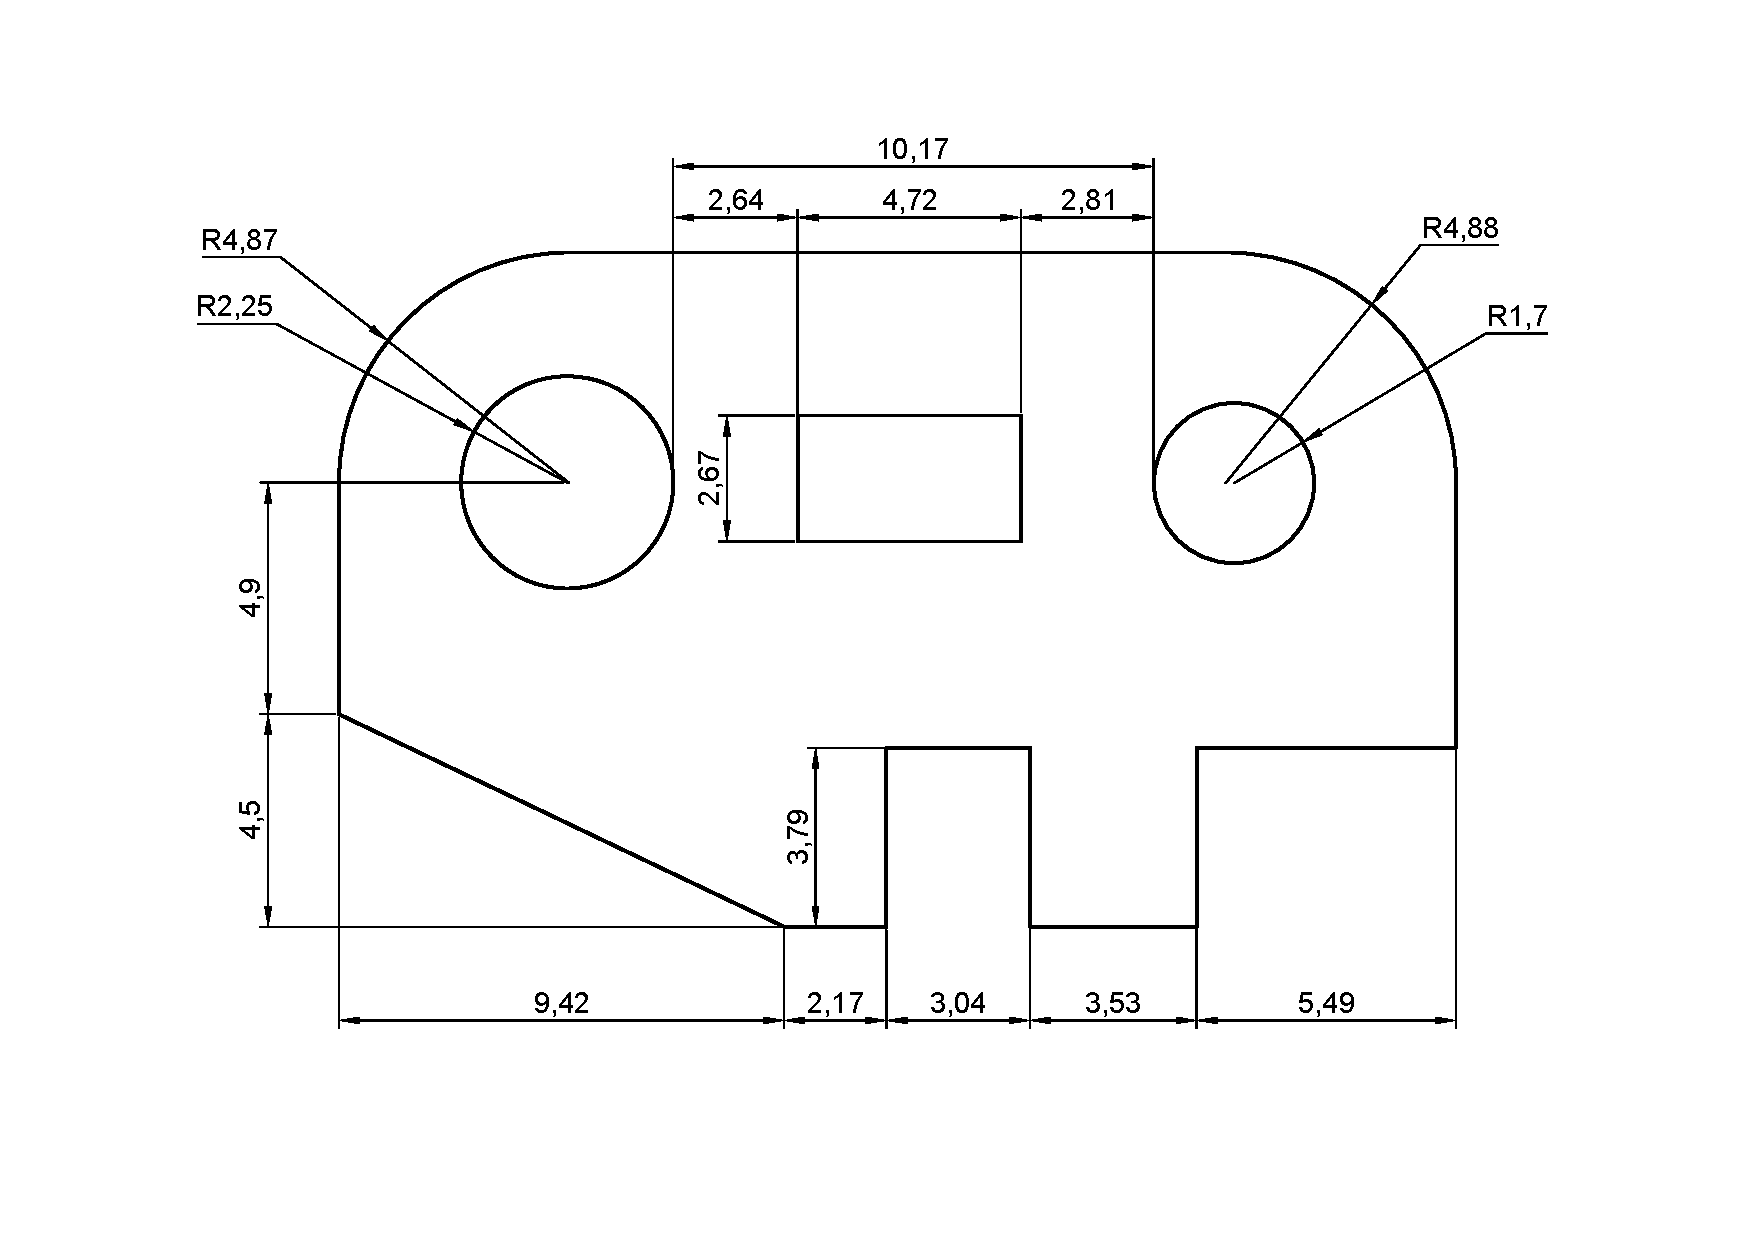
\includegraphics[width=.89\linewidth]{Meow.pdf}
	\caption{Kích thước của mẫu đo}
\end{figure}